\documentclass{resume}

\geometry{left=0.50in,right=0.50in,top=0.16in,bottom=0.25in}
\setlist[itemize]{itemsep=0.15ex,topsep=0.15em,leftmargin=1.25pc}

\begin{document}
\pagestyle{empty}
\fontsize{8.6pt}{10pt}\selectfont
\emergencystretch=1.5em
\vspace*{-0.8ex}

\noindent
\begin{minipage}[t]{0.74\textwidth}
  {\LARGE\scshape Qingliu Wu\par}
  \vspace{0.6ex}
  {\ttfamily\normalsize
    \phone{17353675760} \textperiodcentered\
    \email{wql@bupt.edu.cn} \textperiodcentered\
    \github[micuks]{https://github.com/micuks}\par
  }
\end{minipage}\hfill
\makebox[0pt][r]{\raisebox{-7ex}[0pt][0pt]{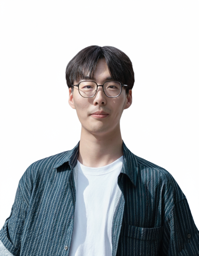
\includegraphics[width=2.2cm,clip,trim=0 57 0 0]{selfie.png}}}
\vspace{-0.2ex}

\section{Education}
\datedsubsection{\textbf{Beijing University of Posts and Telecommunications (BUPT)}}{09/2024 -- 06/2027}
\begin{itemize}[parsep=0.25ex]
  \item M.Sc. Candidate in Computer Science; \textbf{National Scholarship (2024--2025)}; AI4DB research at the IDMG Lab under Prof. Yingxia Shao.
\end{itemize}
\datedsubsection{\textbf{BUPT}}{09/2020 -- 06/2024}
\begin{itemize}[parsep=0.25ex]
  \item B.Eng. in Computer Science (Experimental Class); score 91.91, ranked 29/422 (top 6.56\%).
\end{itemize}

\section{Internship Experience}

\role{Qwen3.8-Next / Qwen3.6 Training Optimization \textnormal{\normalfont\itshape{ | FP8 / MegaMoE / Megatron}}}{2026.10 -- Present}
{\small\itshape Kuaishou, Algorithm Engine Dept., Training Engine Team | AI Infra\par}
\begin{itemize}[parsep=0.25ex]
  \item \textbf{FP8 memory \& tensor lifecycle:} For Qwen3.8-Next / Qwen3.6 (GDN+Full Attn+256-expert MoE+MTP) 262K FP8 training, fixed layout mismatches via on-demand transient non-MoE weight columns (skipping post-gather transposes), dual-quant \texttt{O-proj} activation release, and dropping 2 GiB dead expert columns; with CP-local RoPE, unified GDN+MoE checkpointing, and light Attn recompute, cut 35B-A3B 32-H200 peak memory 26.0\% (69.7 $\to$ 51.6 GiB) at matched parallelism.
  \item \textbf{End-to-end MegaMoE integration \& optimization:} Integrated CuTe-DSL MegaMoE into Megatron for Qwen3.6 and led migration to Qwen3.8-Next: shifted 8-row interleaved \texttt{fc1} quantization to the optimizer boundary (1B FP8 AG preserved; reversed registration offsetting DDP order for zero-copy forward views replacing 160+ per-step requants), with shared fwd/bwd workspaces, Triton compact routing, epilogue \texttt{main\_grad} writes, GPU-only overflow checks, and Triton tiled transposes.
  \item \textbf{Long-context kernels \& operator fusion:} Built single-pass 248K Linear CE direct \texttt{main\_grad} writes (1.62$\times$) with SFT valid-label compaction and CP balancing; fused QK-Norm+partial mRoPE (3.09$\times$) and optimized GDN replay/\texttt{tile16}/AllToAll fusion; integrated native SM90 two-stage TMA Attention bwd (15\%--21\% faster than FA3; \texttt{H=1} saves 1.1 GiB), cutting 32-H200 262K step time 15.9\% (23.43 $\to$ 19.72 s) with 23-step parity.
\end{itemize}

\role{Keye Multimodal Model Pre-training Infrastructure \textnormal{\normalfont\itshape{ | Megatron}}}{2026.05 -- 2026.10}
{\small\itshape Kuaishou, Kling AI Business Unit | AI Infra\par}
\begin{itemize}[parsep=0.25ex]
  \item \textbf{Long-context training architecture:} Implemented Context Parallel for Causal-ViT with Ulysses All-to-All for GDN and cross-shard MoDA halos. Unified mixed image-video sharding and loss reduction through a padding-free \texttt{PackedVisionLayout}, removed the CP batch-size-1 restriction, and scaled CP8 samples from 131K to 2M visual tokens.
  \item \textbf{1K-GPU training stability:} Supported Stage-2 training on 1,024 GPUs (CP8$\times$DP128, GBS 2,048, up to 2,048 frames/$\sim$2M visual tokens per sample). Traced a CP8 hang to empty short-video shards skipping a backward All-Reduce, anchored the graph to align collective sequences across ranks, and observed no recurrence in 1K-GPU training after the fix.
  \item \textbf{MoDA compute optimization:} Replaced a launch-bound per-frame Python loop with cross-frame batching for 5.4$\times$/1.28$\times$ single-layer/end-to-end speedups. Further designed chunked packed MoDA, staging QKV, gate, attention, and output intermediates against backward recompute for another 3.36$\times$ per layer while still training at 2M tokens; aligned BF16 single-layer outputs and forward/backward gradients, with no regression in real-training evaluation.
  \item \textbf{Engineering correctness:} Built a real-training CP=1 golden reference and compared CP=N forward outputs, input gradients, and every weight gradient; a full BF16 model passed multi-loss and \texttt{sum}-stress parity plus 8-GPU validation at 4M tokens per step. Also isolated fused-RoPE BF16 NaNs and filed a minimal reproducer upstream (Megatron-LM\#5318).
  \item \textbf{Distributed optimizer:} Root-caused Muon incompatibility with ZeRO-1/2 reduce-scatter: partitioned matrices lacked the complete reduced gradients required by Newton-Schulz. Upstreamed owner-directed sliced propagation and redundant owner updates to DeepSpeed; \textbf{PR\#8141 merged into master}.
\end{itemize}

\role{Flink Large-State Processing Optimization}{2026.03 -- 2026.05}
{\small\itshape Huawei, Computing Product Line | AI Engineer\par}
\begin{itemize}[parsep=0.25ex]
  \item \textbf{State-access pipeline:} For Flink 1.16.3 + RocksDB large-state workloads, built two-tier Value/Map caches and EMPTY/SINGLE MapState snapshots, then added mailbox batching, MultiGet prefetch, same-key local pre-aggregation, and whole-key MemTable/SST Bloom gates to cut serialization, JNI crossings, and useless block reads.
  \item \textbf{Cross-platform evaluation:} On 100M records, 15 Nexmark queries, and 8 TMs/16 slots, the full stack improved mean per-query throughput over RocksDB StateBackend by 61.77\% on x86 and 42.79\% on Kunpeng; a matched-stack ablation measured an independent 11.08\% Bloom gain, with correctness preserved through invalidation, barrier flushes, and RocksDB as source of truth.
\end{itemize}

\section{Projects}
\role{SQLForge: Execution-Feedback Post-training for Text-to-SQL Agents \textnormal{\normalfont\itshape{ | QLoRA / GRPO}}}{2026.01 -- 2026.05}
\begin{itemize}[parsep=0.25ex]
  \item \textbf{Execution-feedback post-training:} Generated multi-teacher ReAct trajectories with every observation rewritten from real SQLite results; trained ReAct SFT with DeepSpeed ZeRO-2 and built a GRPO loop combining format, validity, structure, partial-execution, and final-correctness rewards.
  \item \textbf{Interactive self-correction:} Designed Direct SQL with Interactive ReAct fallback after execution failure, executing drafts in a sandbox and continuing from observations; reached 78.6\% Execution Match on 200 Spider validation examples, +6.9pp over ReAct SFT direct-only (71.7\%).
\end{itemize}


\section{Research Experience}
\role{DBPecker: Compound Anomaly Diagnosis for Distributed Databases}{PVLDB 2025 \textperiodcentered\ Co-first Author}
\begin{itemize}[parsep=0.25ex]
  \item \textbf{Compound anomaly diagnosis:} Built a cross-node compound-anomaly graph and used correlation-weighted PageRank to rank $\langle$node, anomaly$\rangle$ pairs by node influence and multi-label anomaly probability; structural-causal interventions identify root-cause metrics across OS and database layers.
\end{itemize}

\section{Skills}
\begin{itemize}[parsep=0.25ex]
  \item \textbf{LLM Systems}: Megatron-LM, DeepSpeed, Transformer Engine FP8, Triton, PyTorch, vLLM; SFT, GRPO, ReAct Agents; 1K-GPU pre-training performance/memory and kernel optimization.
  \item \textbf{Languages \& Tools}: C++/Python; familiar with Java/Go/Rust; Linux, Git, Docker, and CMake.
  \item \textbf{English \& Award}: IELTS 7.5 (Reading/Listening 8.5), CET-6 594; National First Prize in Baidu Apollo Autonomous Driving Simulation.
\end{itemize}

\end{document}
